\problemname{The Town Square}

The archaeologist Arvid is searching for an unknown town square from the Iron Age somewhere in central Sweden.
He has mapped a number of farms that existed in the area, and has concluded that the town square must have been at the same distance from each of the farms.

The area Arvid is investigating can be represented by a grid with $N$ rows and $M$ columns.
It takes one minute for an Iron Age person to travel between two adjacent cells.
Two cells are adjacent if they share one of their four sides.

You are given a map of the grid that marks all positions of farms.
It is known that it takes the same amount of time to travel from each of the farms to the town square.
Your task is to find which cells the town square could have been located at.

\section*{Input}
The first line contains the integers $N$ and $M$ ($1 \leq N,M \leq 10$), the number of rows and columns in the grid.

The following $N$ lines each contain a string of length $M$, consisting of the characters `\verb|.|' and `\verb|*|'.
These are the rows of the grid.
The character `\verb|*|' means that there is a farm at the corresponding position in the grid, and `\verb|.|' means that there is not.

There will be at least two farms in the grid.
The input has been generated such that there is always at least one cell where the town square could have been.

\section*{Output}
Print $N$ lines with a string of length $M$ on each line, a copy of the grid from the input but where you have marked with `\verb|X|' the cells where the town square could have been located.

\section*{Scoring}
Your solution will be tested on a set of test groups.
To earn points for a group, you must pass all test cases in that group.


\noindent
\begin{tabular}{| l | l | p{12cm} |}
  \hline
  \textbf{Group} & \textbf{Points} & \textbf{Constraints} \\ \hline
  $1$      & $31$      & $N = 1$ \\ \hline
  $2$      & $21$      & There are exactly $4$ farms that all lie on the corners of the same rectangle. \\ \hline
  $3$      & $48$      & No additional constraints. \\ \hline
\end{tabular}


\section*{Explanation of Samples}

In sample $1$, the farms are in the first and last columns of the top row.
The third cell on the top row is two minutes from both farms.
All cells directly below it have the same distance to both farms: go up to the top row and then equally far to the left or right.

In sample $2$, the farms are in the first and seventh columns.
The cell in the fourth column is three minutes from both farms.
No other cell on the row has the same distance to both.


\begin{figure}[h]
  \centering
  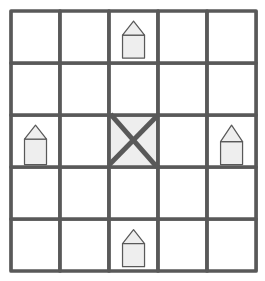
\includegraphics[width=0.2\textwidth]{sample3.png}

  \vspace{0.5cm}
  \parbox{\linewidth}{\centering
  The picture shows the solution to sample $3$. The marked cell in the center is the only possible position for the town square. It takes two minutes to travel from each farm to this cell.
  }
\end{figure}
